\documentclass[twoside]{book}

% Packages required by doxygen
\usepackage{fixltx2e}
\usepackage{calc}
\usepackage{doxygen}
\usepackage[export]{adjustbox} % also loads graphicx
\usepackage{graphicx}
\usepackage[utf8]{inputenc}
\usepackage{makeidx}
\usepackage{multicol}
\usepackage{multirow}
\PassOptionsToPackage{warn}{textcomp}
\usepackage{textcomp}
\usepackage[nointegrals]{wasysym}
\usepackage[table]{xcolor}

% Font selection
\usepackage[T1]{fontenc}
\usepackage[scaled=.90]{helvet}
\usepackage{courier}
\usepackage{amssymb}
\usepackage{sectsty}
\renewcommand{\familydefault}{\sfdefault}
\allsectionsfont{%
  \fontseries{bc}\selectfont%
  \color{darkgray}%
}
\renewcommand{\DoxyLabelFont}{%
  \fontseries{bc}\selectfont%
  \color{darkgray}%
}
\newcommand{\+}{\discretionary{\mbox{\scriptsize$\hookleftarrow$}}{}{}}

% Page & text layout
\usepackage{geometry}
\geometry{%
  a4paper,%
  top=2.5cm,%
  bottom=2.5cm,%
  left=2.5cm,%
  right=2.5cm%
}
\tolerance=750
\hfuzz=15pt
\hbadness=750
\setlength{\emergencystretch}{15pt}
\setlength{\parindent}{0cm}
\setlength{\parskip}{3ex plus 2ex minus 2ex}
\makeatletter
\renewcommand{\paragraph}{%
  \@startsection{paragraph}{4}{0ex}{-1.0ex}{1.0ex}{%
    \normalfont\normalsize\bfseries\SS@parafont%
  }%
}
\renewcommand{\subparagraph}{%
  \@startsection{subparagraph}{5}{0ex}{-1.0ex}{1.0ex}{%
    \normalfont\normalsize\bfseries\SS@subparafont%
  }%
}
\makeatother

% Headers & footers
\usepackage{fancyhdr}
\pagestyle{fancyplain}
\fancyhead[LE]{\fancyplain{}{\bfseries\thepage}}
\fancyhead[CE]{\fancyplain{}{}}
\fancyhead[RE]{\fancyplain{}{\bfseries\leftmark}}
\fancyhead[LO]{\fancyplain{}{\bfseries\rightmark}}
\fancyhead[CO]{\fancyplain{}{}}
\fancyhead[RO]{\fancyplain{}{\bfseries\thepage}}
\fancyfoot[LE]{\fancyplain{}{}}
\fancyfoot[CE]{\fancyplain{}{}}
\fancyfoot[RE]{\fancyplain{}{\bfseries\scriptsize Generated by Doxygen }}
\fancyfoot[LO]{\fancyplain{}{\bfseries\scriptsize Generated by Doxygen }}
\fancyfoot[CO]{\fancyplain{}{}}
\fancyfoot[RO]{\fancyplain{}{}}
\renewcommand{\footrulewidth}{0.4pt}
\renewcommand{\chaptermark}[1]{%
  \markboth{#1}{}%
}
\renewcommand{\sectionmark}[1]{%
  \markright{\thesection\ #1}%
}

% Indices & bibliography
\usepackage{natbib}
\usepackage[titles]{tocloft}
\setcounter{tocdepth}{3}
\setcounter{secnumdepth}{5}
\makeindex

% Hyperlinks (required, but should be loaded last)
\usepackage{ifpdf}
\ifpdf
  \usepackage[pdftex,pagebackref=true]{hyperref}
\else
  \usepackage[ps2pdf,pagebackref=true]{hyperref}
\fi
\hypersetup{%
  colorlinks=true,%
  linkcolor=blue,%
  citecolor=blue,%
  unicode%
}

% Custom commands
\newcommand{\clearemptydoublepage}{%
  \newpage{\pagestyle{empty}\cleardoublepage}%
}

\usepackage{caption}
\captionsetup{labelsep=space,justification=centering,font={bf},singlelinecheck=off,skip=4pt,position=top}

%===== C O N T E N T S =====

\begin{document}

% Titlepage & ToC
\hypersetup{pageanchor=false,
             bookmarksnumbered=true,
             pdfencoding=unicode
            }
\pagenumbering{roman}
\begin{titlepage}
\vspace*{7cm}
\begin{center}%
{\Large U\+I\+Test\+\_\+qwidget }\\
\vspace*{1cm}
{\large Generated by Doxygen 1.8.11}\\
\end{center}
\end{titlepage}
\clearemptydoublepage
\tableofcontents
\clearemptydoublepage
\pagenumbering{arabic}
\hypersetup{pageanchor=true}

%--- Begin generated contents ---
\chapter{U\+I\+Test\+\_\+qwidget}
\label{md_README}
\hypertarget{md_README}{}
Playing around with some old friend qwidgets 
\chapter{Hierarchical Index}
\section{Class Hierarchy}
This inheritance list is sorted roughly, but not completely, alphabetically\+:\begin{DoxyCompactList}
\item \contentsline{section}{I\+Business}{\pageref{class_i_business}}{}
\begin{DoxyCompactList}
\item \contentsline{section}{Mock\+Business}{\pageref{class_mock_business}}{}
\end{DoxyCompactList}
\item Q\+Abstract\+List\+Model\begin{DoxyCompactList}
\item \contentsline{section}{Model\+Sections}{\pageref{class_model_sections}}{}
\end{DoxyCompactList}
\item Q\+Main\+Window\begin{DoxyCompactList}
\item \contentsline{section}{Main\+Window}{\pageref{class_main_window}}{}
\end{DoxyCompactList}
\item \contentsline{section}{data\+\_\+model\+:\+:Result\+Code}{\pageref{structdata__model_1_1_result_code}}{}
\item \contentsline{section}{data\+\_\+model\+:\+:Section}{\pageref{classdata__model_1_1_section}}{}
\begin{DoxyCompactList}
\item \contentsline{section}{data\+\_\+model\+:\+:Section\+Alpha}{\pageref{classdata__model_1_1_section_alpha}}{}
\item \contentsline{section}{data\+\_\+model\+:\+:Section\+Beta}{\pageref{classdata__model_1_1_section_beta}}{}
\end{DoxyCompactList}
\end{DoxyCompactList}

\chapter{Class Index}
\section{Class List}
Here are the classes, structs, unions and interfaces with brief descriptions\+:\begin{DoxyCompactList}
\item\contentsline{section}{\hyperlink{class_i_business}{I\+Business} \\*The \hyperlink{class_i_business}{I\+Business} class }{\pageref{class_i_business}}{}
\item\contentsline{section}{\hyperlink{class_main_window}{Main\+Window} \\*The \hyperlink{class_main_window}{Main\+Window} class }{\pageref{class_main_window}}{}
\item\contentsline{section}{\hyperlink{class_mock_business}{Mock\+Business} }{\pageref{class_mock_business}}{}
\item\contentsline{section}{\hyperlink{class_model_sections}{Model\+Sections} \\*The \hyperlink{class_model_sections}{Model\+Sections} class }{\pageref{class_model_sections}}{}
\item\contentsline{section}{\hyperlink{structdata__model_1_1_result_code}{data\+\_\+model\+::\+Result\+Code} \\*The \hyperlink{structdata__model_1_1_result_code}{Result\+Code} struct }{\pageref{structdata__model_1_1_result_code}}{}
\item\contentsline{section}{\hyperlink{classdata__model_1_1_section}{data\+\_\+model\+::\+Section} \\*The \hyperlink{classdata__model_1_1_section}{Section} class }{\pageref{classdata__model_1_1_section}}{}
\item\contentsline{section}{\hyperlink{classdata__model_1_1_section_alpha}{data\+\_\+model\+::\+Section\+Alpha} \\*The \hyperlink{classdata__model_1_1_section_alpha}{Section\+Alpha} class }{\pageref{classdata__model_1_1_section_alpha}}{}
\item\contentsline{section}{\hyperlink{classdata__model_1_1_section_beta}{data\+\_\+model\+::\+Section\+Beta} \\*The \hyperlink{classdata__model_1_1_section_beta}{Section\+Beta} class }{\pageref{classdata__model_1_1_section_beta}}{}
\end{DoxyCompactList}

\chapter{Class Documentation}
\hypertarget{class_i_business}{}\section{I\+Business Class Reference}
\label{class_i_business}\index{I\+Business@{I\+Business}}


The \hyperlink{class_i_business}{I\+Business} class.  




{\ttfamily \#include $<$ibusiness.\+h$>$}



Inheritance diagram for I\+Business\+:
\nopagebreak
\begin{figure}[H]
\begin{center}
\leavevmode
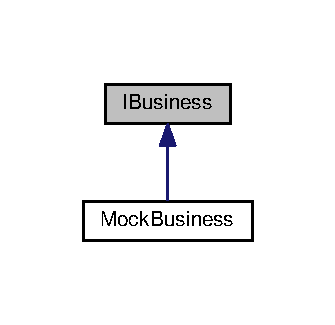
\includegraphics[width=161pt]{class_i_business__inherit__graph}
\end{center}
\end{figure}
\subsection*{Public Member Functions}
\begin{DoxyCompactItemize}
\item 
virtual \hyperlink{class_i_business_a228d92e5f27f5924815f2ba1191084fa}{$\sim$\+I\+Business} ()=default
\begin{DoxyCompactList}\small\item\em $\sim$\+I\+Business \end{DoxyCompactList}\item 
size\+\_\+t \hyperlink{class_i_business_a4df04231605372aac35aaf61f693514f}{Get\+Num\+Section} () const 
\begin{DoxyCompactList}\small\item\em Get\+Num\+Section. \end{DoxyCompactList}\item 
const data\+\_\+model\+::\+Adquisition $\ast$ \hyperlink{class_i_business_a02485d0c224a027b8c4e5f8f79f8bc60}{Get\+Adquisition} () const 
\begin{DoxyCompactList}\small\item\em Get\+Adquisition. \end{DoxyCompactList}\item 
const \hyperlink{classdata__model_1_1_section}{data\+\_\+model\+::\+Section} $\ast$ \hyperlink{class_i_business_ad6e3f210eba0c7517ade17f0d5a904ae}{Get\+Section} (unsigned int) const 
\begin{DoxyCompactList}\small\item\em Get\+Section. \end{DoxyCompactList}\item 
virtual void \hyperlink{class_i_business_a26e62b89d3d994dde2b0b528ee3ccf09}{Process\+New\+Adquisition} ()=0\hypertarget{class_i_business_a26e62b89d3d994dde2b0b528ee3ccf09}{}\label{class_i_business_a26e62b89d3d994dde2b0b528ee3ccf09}

\begin{DoxyCompactList}\small\item\em Process\+New\+Adquisition. \end{DoxyCompactList}\end{DoxyCompactItemize}
\subsection*{Protected Member Functions}
\begin{DoxyCompactItemize}
\item 
\hyperlink{class_i_business_ad8f2b5adfe83996565ea10b416c4f36e}{I\+Business} ()\hypertarget{class_i_business_ad8f2b5adfe83996565ea10b416c4f36e}{}\label{class_i_business_ad8f2b5adfe83996565ea10b416c4f36e}

\begin{DoxyCompactList}\small\item\em \hyperlink{class_i_business}{I\+Business}. \end{DoxyCompactList}\end{DoxyCompactItemize}
\subsection*{Protected Attributes}
\begin{DoxyCompactItemize}
\item 
data\+\_\+model\+::\+Adquisition \hyperlink{class_i_business_a7065ab5ec85bf94362256617bc1ce14e}{sections\+\_\+}\hypertarget{class_i_business_a7065ab5ec85bf94362256617bc1ce14e}{}\label{class_i_business_a7065ab5ec85bf94362256617bc1ce14e}

\begin{DoxyCompactList}\small\item\em sections\+\_\+ \end{DoxyCompactList}\end{DoxyCompactItemize}


\subsection{Detailed Description}
The \hyperlink{class_i_business}{I\+Business} class. 

\subsection{Constructor \& Destructor Documentation}
\index{I\+Business@{I\+Business}!````~I\+Business@{$\sim$\+I\+Business}}
\index{````~I\+Business@{$\sim$\+I\+Business}!I\+Business@{I\+Business}}
\subsubsection[{\texorpdfstring{$\sim$\+I\+Business()=default}{~IBusiness()=default}}]{\setlength{\rightskip}{0pt plus 5cm}virtual I\+Business\+::$\sim$\+I\+Business (
\begin{DoxyParamCaption}
{}
\end{DoxyParamCaption}
)\hspace{0.3cm}{\ttfamily [virtual]}, {\ttfamily [default]}}\hypertarget{class_i_business_a228d92e5f27f5924815f2ba1191084fa}{}\label{class_i_business_a228d92e5f27f5924815f2ba1191084fa}


$\sim$\+I\+Business 

\begin{DoxyReturn}{Returns}

\end{DoxyReturn}


\subsection{Member Function Documentation}
\index{I\+Business@{I\+Business}!Get\+Adquisition@{Get\+Adquisition}}
\index{Get\+Adquisition@{Get\+Adquisition}!I\+Business@{I\+Business}}
\subsubsection[{\texorpdfstring{Get\+Adquisition() const }{GetAdquisition() const }}]{\setlength{\rightskip}{0pt plus 5cm}const data\+\_\+model\+::\+Adquisition $\ast$ I\+Business\+::\+Get\+Adquisition (
\begin{DoxyParamCaption}
{}
\end{DoxyParamCaption}
) const}\hypertarget{class_i_business_a02485d0c224a027b8c4e5f8f79f8bc60}{}\label{class_i_business_a02485d0c224a027b8c4e5f8f79f8bc60}


Get\+Adquisition. 

\begin{DoxyReturn}{Returns}

\end{DoxyReturn}
\index{I\+Business@{I\+Business}!Get\+Num\+Section@{Get\+Num\+Section}}
\index{Get\+Num\+Section@{Get\+Num\+Section}!I\+Business@{I\+Business}}
\subsubsection[{\texorpdfstring{Get\+Num\+Section() const }{GetNumSection() const }}]{\setlength{\rightskip}{0pt plus 5cm}size\+\_\+t I\+Business\+::\+Get\+Num\+Section (
\begin{DoxyParamCaption}
{}
\end{DoxyParamCaption}
) const}\hypertarget{class_i_business_a4df04231605372aac35aaf61f693514f}{}\label{class_i_business_a4df04231605372aac35aaf61f693514f}


Get\+Num\+Section. 

\begin{DoxyReturn}{Returns}

\end{DoxyReturn}
\index{I\+Business@{I\+Business}!Get\+Section@{Get\+Section}}
\index{Get\+Section@{Get\+Section}!I\+Business@{I\+Business}}
\subsubsection[{\texorpdfstring{Get\+Section(unsigned int) const }{GetSection(unsigned int) const }}]{\setlength{\rightskip}{0pt plus 5cm}const {\bf data\+\_\+model\+::\+Section} $\ast$ I\+Business\+::\+Get\+Section (
\begin{DoxyParamCaption}
\item[{unsigned int}]{i}
\end{DoxyParamCaption}
) const}\hypertarget{class_i_business_ad6e3f210eba0c7517ade17f0d5a904ae}{}\label{class_i_business_ad6e3f210eba0c7517ade17f0d5a904ae}


Get\+Section. 

\begin{DoxyReturn}{Returns}

\end{DoxyReturn}


The documentation for this class was generated from the following files\+:\begin{DoxyCompactItemize}
\item 
ibusiness.\+h\item 
ibusiness.\+cpp\end{DoxyCompactItemize}

\hypertarget{class_main_window}{}\section{Main\+Window Class Reference}
\label{class_main_window}\index{Main\+Window@{Main\+Window}}


The \hyperlink{class_main_window}{Main\+Window} class.  




{\ttfamily \#include $<$mainwindow.\+h$>$}



Inheritance diagram for Main\+Window\+:
\nopagebreak
\begin{figure}[H]
\begin{center}
\leavevmode
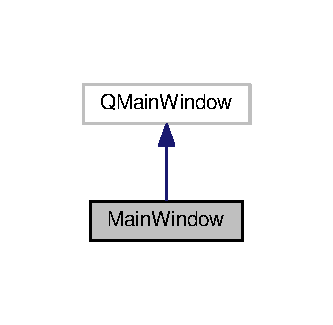
\includegraphics[width=160pt]{class_main_window__inherit__graph}
\end{center}
\end{figure}


Collaboration diagram for Main\+Window\+:
\nopagebreak
\begin{figure}[H]
\begin{center}
\leavevmode
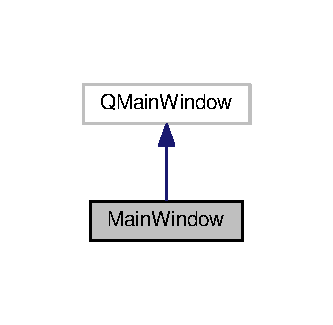
\includegraphics[width=160pt]{class_main_window__coll__graph}
\end{center}
\end{figure}
\subsection*{Signals}
\begin{DoxyCompactItemize}
\item 
void \hyperlink{class_main_window_af1c023e4354a163ebd130aa55aad2583}{New\+Result} ()\hypertarget{class_main_window_af1c023e4354a163ebd130aa55aad2583}{}\label{class_main_window_af1c023e4354a163ebd130aa55aad2583}

\begin{DoxyCompactList}\small\item\em New\+Result. \end{DoxyCompactList}\end{DoxyCompactItemize}
\subsection*{Public Member Functions}
\begin{DoxyCompactItemize}
\item 
\hyperlink{class_main_window_a996c5a2b6f77944776856f08ec30858d}{Main\+Window} (Q\+Widget $\ast$parent=nullptr)
\begin{DoxyCompactList}\small\item\em \hyperlink{class_main_window}{Main\+Window}. \end{DoxyCompactList}\item 
\hyperlink{class_main_window_ae98d00a93bc118200eeef9f9bba1dba7}{$\sim$\+Main\+Window} ()
\begin{DoxyCompactList}\small\item\em \hyperlink{class_main_window}{Main\+Window}. \end{DoxyCompactList}\item 
void \hyperlink{class_main_window_ae17ca5d5ac5314191edb702fadcbb101}{Initialize\+Model} ()\hypertarget{class_main_window_ae17ca5d5ac5314191edb702fadcbb101}{}\label{class_main_window_ae17ca5d5ac5314191edb702fadcbb101}

\begin{DoxyCompactList}\small\item\em Initialize\+Model. \end{DoxyCompactList}\item 
void \hyperlink{class_main_window_af8cad047758d58a96e68bdbe3ed7d99f}{Initialize\+UI} ()\hypertarget{class_main_window_af8cad047758d58a96e68bdbe3ed7d99f}{}\label{class_main_window_af8cad047758d58a96e68bdbe3ed7d99f}

\begin{DoxyCompactList}\small\item\em Initialize\+UI. \end{DoxyCompactList}\end{DoxyCompactItemize}


\subsection{Detailed Description}
The \hyperlink{class_main_window}{Main\+Window} class. 

\subsection{Constructor \& Destructor Documentation}
\index{Main\+Window@{Main\+Window}!Main\+Window@{Main\+Window}}
\index{Main\+Window@{Main\+Window}!Main\+Window@{Main\+Window}}
\subsubsection[{\texorpdfstring{Main\+Window(\+Q\+Widget $\ast$parent=nullptr)}{MainWindow(QWidget *parent=nullptr)}}]{\setlength{\rightskip}{0pt plus 5cm}Main\+Window\+::\+Main\+Window (
\begin{DoxyParamCaption}
\item[{Q\+Widget $\ast$}]{parent = {\ttfamily nullptr}}
\end{DoxyParamCaption}
)}\hypertarget{class_main_window_a996c5a2b6f77944776856f08ec30858d}{}\label{class_main_window_a996c5a2b6f77944776856f08ec30858d}


\hyperlink{class_main_window}{Main\+Window}. 


\begin{DoxyParams}{Parameters}
{\em parent} & \\
\hline
\end{DoxyParams}
\index{Main\+Window@{Main\+Window}!````~Main\+Window@{$\sim$\+Main\+Window}}
\index{````~Main\+Window@{$\sim$\+Main\+Window}!Main\+Window@{Main\+Window}}
\subsubsection[{\texorpdfstring{$\sim$\+Main\+Window()}{~MainWindow()}}]{\setlength{\rightskip}{0pt plus 5cm}Main\+Window\+::$\sim$\+Main\+Window (
\begin{DoxyParamCaption}
{}
\end{DoxyParamCaption}
)}\hypertarget{class_main_window_ae98d00a93bc118200eeef9f9bba1dba7}{}\label{class_main_window_ae98d00a93bc118200eeef9f9bba1dba7}


\hyperlink{class_main_window}{Main\+Window}. 


\begin{DoxyParams}{Parameters}
{\em parent} & \\
\hline
\end{DoxyParams}


The documentation for this class was generated from the following files\+:\begin{DoxyCompactItemize}
\item 
mainwindow.\+h\item 
mainwindow.\+cpp\end{DoxyCompactItemize}

\hypertarget{class_mock_business}{}\section{Mock\+Business Class Reference}
\label{class_mock_business}\index{Mock\+Business@{Mock\+Business}}


Inheritance diagram for Mock\+Business\+:
\nopagebreak
\begin{figure}[H]
\begin{center}
\leavevmode
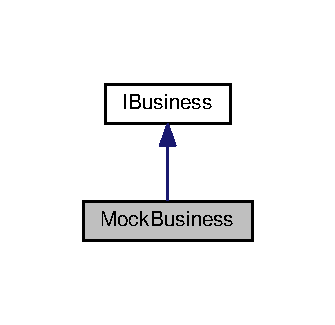
\includegraphics[width=161pt]{class_mock_business__inherit__graph}
\end{center}
\end{figure}


Collaboration diagram for Mock\+Business\+:
\nopagebreak
\begin{figure}[H]
\begin{center}
\leavevmode
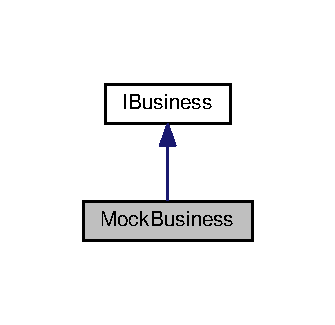
\includegraphics[width=161pt]{class_mock_business__coll__graph}
\end{center}
\end{figure}
\subsection*{Public Member Functions}
\begin{DoxyCompactItemize}
\item 
void \hyperlink{class_mock_business_ad9d35921a0b2ed09268197273d9c10f3}{Process\+New\+Adquisition} () override\hypertarget{class_mock_business_ad9d35921a0b2ed09268197273d9c10f3}{}\label{class_mock_business_ad9d35921a0b2ed09268197273d9c10f3}

\begin{DoxyCompactList}\small\item\em Process\+New\+Adquisition. \end{DoxyCompactList}\end{DoxyCompactItemize}
\subsection*{Additional Inherited Members}


The documentation for this class was generated from the following files\+:\begin{DoxyCompactItemize}
\item 
mocks/mockbusiness.\+h\item 
mocks/mockbusiness.\+cpp\end{DoxyCompactItemize}

\hypertarget{class_model_sections}{}\section{Model\+Sections Class Reference}
\label{class_model_sections}\index{Model\+Sections@{Model\+Sections}}


The \hyperlink{class_model_sections}{Model\+Sections} class.  




{\ttfamily \#include $<$modelsections.\+h$>$}



Inheritance diagram for Model\+Sections\+:
\nopagebreak
\begin{figure}[H]
\begin{center}
\leavevmode
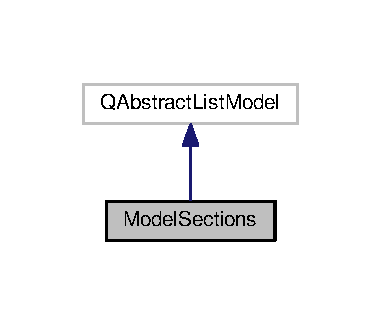
\includegraphics[width=183pt]{class_model_sections__inherit__graph}
\end{center}
\end{figure}


Collaboration diagram for Model\+Sections\+:
\nopagebreak
\begin{figure}[H]
\begin{center}
\leavevmode
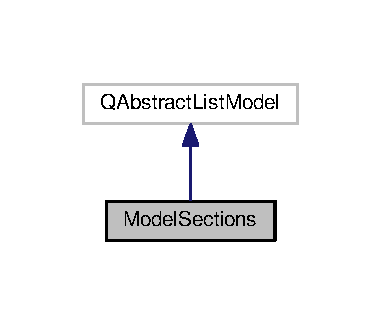
\includegraphics[width=183pt]{class_model_sections__coll__graph}
\end{center}
\end{figure}
\subsection*{Public Slots}
\begin{DoxyCompactItemize}
\item 
void \hyperlink{class_model_sections_ae6b216f4975cda057d69628ef9ee5e63}{On\+New\+Result} ()\hypertarget{class_model_sections_ae6b216f4975cda057d69628ef9ee5e63}{}\label{class_model_sections_ae6b216f4975cda057d69628ef9ee5e63}

\begin{DoxyCompactList}\small\item\em On\+New\+Result. \end{DoxyCompactList}\end{DoxyCompactItemize}
\subsection*{Public Member Functions}
\begin{DoxyCompactItemize}
\item 
\hyperlink{class_model_sections_a50d8b404462b552f688abab957e32d79}{Model\+Sections} (Q\+Object $\ast$parent=nullptr)
\begin{DoxyCompactList}\small\item\em \hyperlink{class_model_sections}{Model\+Sections}. \end{DoxyCompactList}\item 
int \hyperlink{class_model_sections_ab23527240092e094ed0a135470fe2676}{row\+Count} (const Q\+Model\+Index \&parent=Q\+Model\+Index()) const override
\begin{DoxyCompactList}\small\item\em row\+Count \end{DoxyCompactList}\item 
Q\+Variant \hyperlink{class_model_sections_a3af1ab537c7c32526057ed46e6ac72d1}{data} (const Q\+Model\+Index \&index, int role=Qt\+::\+Display\+Role) const override
\begin{DoxyCompactList}\small\item\em data \end{DoxyCompactList}\item 
const data\+\_\+model\+::\+Adquisition $\ast$ \hyperlink{class_model_sections_a1fbcda847987cd5c44b0c542802c44c7}{Get\+Adquisition} ()
\begin{DoxyCompactList}\small\item\em Get\+Adquisition. \end{DoxyCompactList}\end{DoxyCompactItemize}


\subsection{Detailed Description}
The \hyperlink{class_model_sections}{Model\+Sections} class. 

\subsection{Constructor \& Destructor Documentation}
\index{Model\+Sections@{Model\+Sections}!Model\+Sections@{Model\+Sections}}
\index{Model\+Sections@{Model\+Sections}!Model\+Sections@{Model\+Sections}}
\subsubsection[{\texorpdfstring{Model\+Sections(\+Q\+Object $\ast$parent=nullptr)}{ModelSections(QObject *parent=nullptr)}}]{\setlength{\rightskip}{0pt plus 5cm}Model\+Sections\+::\+Model\+Sections (
\begin{DoxyParamCaption}
\item[{Q\+Object $\ast$}]{parent = {\ttfamily nullptr}}
\end{DoxyParamCaption}
)\hspace{0.3cm}{\ttfamily [explicit]}}\hypertarget{class_model_sections_a50d8b404462b552f688abab957e32d79}{}\label{class_model_sections_a50d8b404462b552f688abab957e32d79}


\hyperlink{class_model_sections}{Model\+Sections}. 


\begin{DoxyParams}{Parameters}
{\em parent} & \\
\hline
\end{DoxyParams}


\subsection{Member Function Documentation}
\index{Model\+Sections@{Model\+Sections}!data@{data}}
\index{data@{data}!Model\+Sections@{Model\+Sections}}
\subsubsection[{\texorpdfstring{data(const Q\+Model\+Index \&index, int role=\+Qt\+::\+Display\+Role) const override}{data(const QModelIndex &index, int role=Qt::DisplayRole) const override}}]{\setlength{\rightskip}{0pt plus 5cm}Q\+Variant Model\+Sections\+::data (
\begin{DoxyParamCaption}
\item[{const Q\+Model\+Index \&}]{index, }
\item[{int}]{role = {\ttfamily Qt\+:\+:DisplayRole}}
\end{DoxyParamCaption}
) const\hspace{0.3cm}{\ttfamily [override]}}\hypertarget{class_model_sections_a3af1ab537c7c32526057ed46e6ac72d1}{}\label{class_model_sections_a3af1ab537c7c32526057ed46e6ac72d1}


data 


\begin{DoxyParams}{Parameters}
{\em index} & \\
\hline
{\em role} & \\
\hline
\end{DoxyParams}
\begin{DoxyReturn}{Returns}

\end{DoxyReturn}
\index{Model\+Sections@{Model\+Sections}!Get\+Adquisition@{Get\+Adquisition}}
\index{Get\+Adquisition@{Get\+Adquisition}!Model\+Sections@{Model\+Sections}}
\subsubsection[{\texorpdfstring{Get\+Adquisition()}{GetAdquisition()}}]{\setlength{\rightskip}{0pt plus 5cm}const data\+\_\+model\+::\+Adquisition$\ast$ Model\+Sections\+::\+Get\+Adquisition (
\begin{DoxyParamCaption}
{}
\end{DoxyParamCaption}
)\hspace{0.3cm}{\ttfamily [inline]}}\hypertarget{class_model_sections_a1fbcda847987cd5c44b0c542802c44c7}{}\label{class_model_sections_a1fbcda847987cd5c44b0c542802c44c7}


Get\+Adquisition. 

\begin{DoxyReturn}{Returns}

\end{DoxyReturn}
\index{Model\+Sections@{Model\+Sections}!row\+Count@{row\+Count}}
\index{row\+Count@{row\+Count}!Model\+Sections@{Model\+Sections}}
\subsubsection[{\texorpdfstring{row\+Count(const Q\+Model\+Index \&parent=\+Q\+Model\+Index()) const override}{rowCount(const QModelIndex &parent=QModelIndex()) const override}}]{\setlength{\rightskip}{0pt plus 5cm}int Model\+Sections\+::row\+Count (
\begin{DoxyParamCaption}
\item[{const Q\+Model\+Index \&}]{parent = {\ttfamily QModelIndex()}}
\end{DoxyParamCaption}
) const\hspace{0.3cm}{\ttfamily [override]}}\hypertarget{class_model_sections_ab23527240092e094ed0a135470fe2676}{}\label{class_model_sections_ab23527240092e094ed0a135470fe2676}


row\+Count 


\begin{DoxyParams}{Parameters}
{\em parent} & \\
\hline
\end{DoxyParams}
\begin{DoxyReturn}{Returns}

\end{DoxyReturn}


The documentation for this class was generated from the following files\+:\begin{DoxyCompactItemize}
\item 
modelsections.\+h\item 
modelsections.\+cpp\end{DoxyCompactItemize}

\hypertarget{structdata__model_1_1_result_code}{}\section{data\+\_\+model\+:\+:Result\+Code Struct Reference}
\label{structdata__model_1_1_result_code}\index{data\+\_\+model\+::\+Result\+Code@{data\+\_\+model\+::\+Result\+Code}}


The \hyperlink{structdata__model_1_1_result_code}{Result\+Code} struct.  




{\ttfamily \#include $<$resultcode.\+h$>$}

\subsection*{Public Types}
\begin{DoxyCompactItemize}
\item 
enum \hyperlink{structdata__model_1_1_result_code_a57c4d467974a51fc8475b9fd2b4ed505}{Code\+Value} \{ {\bfseries k\+Ok} = 0, 
{\bfseries k\+Out\+Of\+Tolerance} = 42, 
{\bfseries k\+Defect} = 43
 \}\hypertarget{structdata__model_1_1_result_code_a57c4d467974a51fc8475b9fd2b4ed505}{}\label{structdata__model_1_1_result_code_a57c4d467974a51fc8475b9fd2b4ed505}
\begin{DoxyCompactList}\small\item\em The Code\+Value enum. \end{DoxyCompactList}
\item 
enum \hyperlink{structdata__model_1_1_result_code_ae2d78d99add6ff3727da0474572464fd}{Code\+Type} \{ {\bfseries k\+Warning}, 
{\bfseries k\+Error}
 \}\hypertarget{structdata__model_1_1_result_code_ae2d78d99add6ff3727da0474572464fd}{}\label{structdata__model_1_1_result_code_ae2d78d99add6ff3727da0474572464fd}
\begin{DoxyCompactList}\small\item\em The Code\+Type enum. \end{DoxyCompactList}
\end{DoxyCompactItemize}
\subsection*{Public Member Functions}
\begin{DoxyCompactItemize}
\item 
\hyperlink{structdata__model_1_1_result_code_a3360d213340fe9acf9220c38c90a9fd4}{Result\+Code} (\hyperlink{structdata__model_1_1_result_code_a57c4d467974a51fc8475b9fd2b4ed505}{Code\+Value}, \hyperlink{structdata__model_1_1_result_code_ae2d78d99add6ff3727da0474572464fd}{Code\+Type})\hypertarget{structdata__model_1_1_result_code_a3360d213340fe9acf9220c38c90a9fd4}{}\label{structdata__model_1_1_result_code_a3360d213340fe9acf9220c38c90a9fd4}

\begin{DoxyCompactList}\small\item\em \hyperlink{structdata__model_1_1_result_code}{Result\+Code}. \end{DoxyCompactList}\end{DoxyCompactItemize}
\subsection*{Public Attributes}
\begin{DoxyCompactItemize}
\item 
\hyperlink{structdata__model_1_1_result_code_a57c4d467974a51fc8475b9fd2b4ed505}{Code\+Value} \hyperlink{structdata__model_1_1_result_code_a497bd5f6f8f5034bf2d8f48ff46a0e18}{value\+\_\+}\hypertarget{structdata__model_1_1_result_code_a497bd5f6f8f5034bf2d8f48ff46a0e18}{}\label{structdata__model_1_1_result_code_a497bd5f6f8f5034bf2d8f48ff46a0e18}

\begin{DoxyCompactList}\small\item\em value\+\_\+ \end{DoxyCompactList}\item 
\hyperlink{structdata__model_1_1_result_code_ae2d78d99add6ff3727da0474572464fd}{Code\+Type} \hyperlink{structdata__model_1_1_result_code_a9aa8ab86645c3b2c62bbc2c356903072}{type\+\_\+}\hypertarget{structdata__model_1_1_result_code_a9aa8ab86645c3b2c62bbc2c356903072}{}\label{structdata__model_1_1_result_code_a9aa8ab86645c3b2c62bbc2c356903072}

\begin{DoxyCompactList}\small\item\em type\+\_\+ \end{DoxyCompactList}\end{DoxyCompactItemize}
\subsection*{Static Public Attributes}
\begin{DoxyCompactItemize}
\item 
static std\+::map$<$ \hyperlink{structdata__model_1_1_result_code_a57c4d467974a51fc8475b9fd2b4ed505}{Code\+Value}, std\+::string $>$ \hyperlink{structdata__model_1_1_result_code_adba7e4beae8cd77b2c9cc807d77f0b19}{k\+Result\+Codes}
\begin{DoxyCompactList}\small\item\em k\+Result\+Codes \end{DoxyCompactList}\end{DoxyCompactItemize}


\subsection{Detailed Description}
The \hyperlink{structdata__model_1_1_result_code}{Result\+Code} struct. 

\subsection{Member Data Documentation}
\index{data\+\_\+model\+::\+Result\+Code@{data\+\_\+model\+::\+Result\+Code}!k\+Result\+Codes@{k\+Result\+Codes}}
\index{k\+Result\+Codes@{k\+Result\+Codes}!data\+\_\+model\+::\+Result\+Code@{data\+\_\+model\+::\+Result\+Code}}
\subsubsection[{\texorpdfstring{k\+Result\+Codes}{kResultCodes}}]{\setlength{\rightskip}{0pt plus 5cm}std\+::map$<$ {\bf Result\+Code\+::\+Code\+Value}, std\+::string $>$ data\+\_\+model\+::\+Result\+Code\+::k\+Result\+Codes\hspace{0.3cm}{\ttfamily [static]}}\hypertarget{structdata__model_1_1_result_code_adba7e4beae8cd77b2c9cc807d77f0b19}{}\label{structdata__model_1_1_result_code_adba7e4beae8cd77b2c9cc807d77f0b19}
{\bfseries Initial value\+:}
\begin{DoxyCode}
= \{
    \{CodeValue::kOutOfTolerance,
     \textcolor{stringliteral}{"CD Out of tolerance"}\},       
    \{CodeValue::kDefect, \textcolor{stringliteral}{"Defect"}\} 
\}
\end{DoxyCode}


k\+Result\+Codes 



The documentation for this struct was generated from the following files\+:\begin{DoxyCompactItemize}
\item 
model/resultcode.\+h\item 
model/resultcode.\+cpp\end{DoxyCompactItemize}

\hypertarget{classdata__model_1_1_section}{}\section{data\+\_\+model\+:\+:Section Class Reference}
\label{classdata__model_1_1_section}\index{data\+\_\+model\+::\+Section@{data\+\_\+model\+::\+Section}}


The \hyperlink{classdata__model_1_1_section}{Section} class.  




{\ttfamily \#include $<$section.\+h$>$}



Inheritance diagram for data\+\_\+model\+:\+:Section\+:
\nopagebreak
\begin{figure}[H]
\begin{center}
\leavevmode
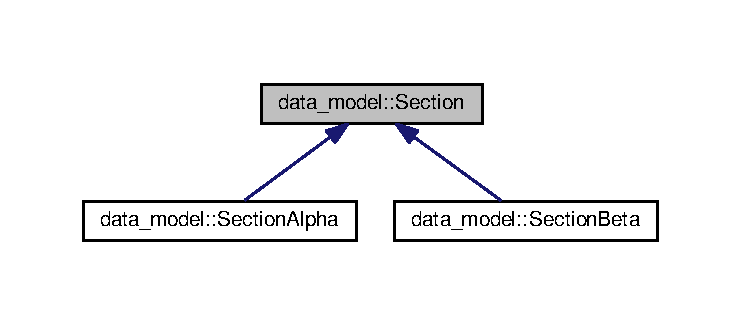
\includegraphics[width=350pt]{classdata__model_1_1_section__inherit__graph}
\end{center}
\end{figure}
\subsection*{Public Types}
\begin{DoxyCompactItemize}
\item 
enum \hyperlink{classdata__model_1_1_section_acba8f1759f6c20b81bed2d4a1178a155}{Section\+Type} \{ {\bfseries k\+Alpha}, 
{\bfseries k\+Beta}
 \}\hypertarget{classdata__model_1_1_section_acba8f1759f6c20b81bed2d4a1178a155}{}\label{classdata__model_1_1_section_acba8f1759f6c20b81bed2d4a1178a155}
\begin{DoxyCompactList}\small\item\em The Section\+Type enum. \end{DoxyCompactList}
\end{DoxyCompactItemize}
\subsection*{Public Member Functions}
\begin{DoxyCompactItemize}
\item 
virtual \hyperlink{classdata__model_1_1_section_a55c82d3aed3c42a5fce529234db90d2e}{$\sim$\+Section} ()=default
\begin{DoxyCompactList}\small\item\em $\sim$\+Section \end{DoxyCompactList}\item 
unsigned int \hyperlink{classdata__model_1_1_section_a83603e6c65fb2c9c94db69bffe3b9410}{Get\+Length} () const 
\begin{DoxyCompactList}\small\item\em Get\+Length. \end{DoxyCompactList}\item 
unsigned int \hyperlink{classdata__model_1_1_section_aac5fb205cbeea09302d1aa136967d1eb}{Get\+OD} () const 
\begin{DoxyCompactList}\small\item\em Get\+OD. \end{DoxyCompactList}\item 
virtual \hyperlink{classdata__model_1_1_section_acba8f1759f6c20b81bed2d4a1178a155}{Section\+Type} \hyperlink{classdata__model_1_1_section_a06487a79e538e1849bb1838cf6a0875b}{Get\+Section\+Type} () const =0
\begin{DoxyCompactList}\small\item\em Get\+Section\+Type. \end{DoxyCompactList}\item 
void \hyperlink{classdata__model_1_1_section_aa15a407b629dfe483c31864f7e4b682a}{Set\+Length} (unsigned int)\hypertarget{classdata__model_1_1_section_aa15a407b629dfe483c31864f7e4b682a}{}\label{classdata__model_1_1_section_aa15a407b629dfe483c31864f7e4b682a}

\begin{DoxyCompactList}\small\item\em Set\+Length. \end{DoxyCompactList}\item 
void \hyperlink{classdata__model_1_1_section_a4102c89fa4727b923d31348d33bd935b}{Set\+OD} (unsigned int)\hypertarget{classdata__model_1_1_section_a4102c89fa4727b923d31348d33bd935b}{}\label{classdata__model_1_1_section_a4102c89fa4727b923d31348d33bd935b}

\begin{DoxyCompactList}\small\item\em Set\+OD. \end{DoxyCompactList}\end{DoxyCompactItemize}
\subsection*{Protected Attributes}
\begin{DoxyCompactItemize}
\item 
unsigned int \hyperlink{classdata__model_1_1_section_a760ab6377b70622fd7973a02c455257a}{length\+\_\+}\hypertarget{classdata__model_1_1_section_a760ab6377b70622fd7973a02c455257a}{}\label{classdata__model_1_1_section_a760ab6377b70622fd7973a02c455257a}

\begin{DoxyCompactList}\small\item\em od\+\_\+ \end{DoxyCompactList}\item 
unsigned int \hyperlink{classdata__model_1_1_section_a222a8b4264e1fe61351107dedac716f3}{od\+\_\+}\hypertarget{classdata__model_1_1_section_a222a8b4264e1fe61351107dedac716f3}{}\label{classdata__model_1_1_section_a222a8b4264e1fe61351107dedac716f3}

\begin{DoxyCompactList}\small\item\em od\+\_\+ \end{DoxyCompactList}\end{DoxyCompactItemize}


\subsection{Detailed Description}
The \hyperlink{classdata__model_1_1_section}{Section} class. 

\subsection{Constructor \& Destructor Documentation}
\index{data\+\_\+model\+::\+Section@{data\+\_\+model\+::\+Section}!````~Section@{$\sim$\+Section}}
\index{````~Section@{$\sim$\+Section}!data\+\_\+model\+::\+Section@{data\+\_\+model\+::\+Section}}
\subsubsection[{\texorpdfstring{$\sim$\+Section()=default}{~Section()=default}}]{\setlength{\rightskip}{0pt plus 5cm}virtual data\+\_\+model\+::\+Section\+::$\sim$\+Section (
\begin{DoxyParamCaption}
{}
\end{DoxyParamCaption}
)\hspace{0.3cm}{\ttfamily [virtual]}, {\ttfamily [default]}}\hypertarget{classdata__model_1_1_section_a55c82d3aed3c42a5fce529234db90d2e}{}\label{classdata__model_1_1_section_a55c82d3aed3c42a5fce529234db90d2e}


$\sim$\+Section 

\begin{DoxyReturn}{Returns}

\end{DoxyReturn}


\subsection{Member Function Documentation}
\index{data\+\_\+model\+::\+Section@{data\+\_\+model\+::\+Section}!Get\+Length@{Get\+Length}}
\index{Get\+Length@{Get\+Length}!data\+\_\+model\+::\+Section@{data\+\_\+model\+::\+Section}}
\subsubsection[{\texorpdfstring{Get\+Length() const }{GetLength() const }}]{\setlength{\rightskip}{0pt plus 5cm}unsigned int data\+\_\+model\+::\+Section\+::\+Get\+Length (
\begin{DoxyParamCaption}
{}
\end{DoxyParamCaption}
) const\hspace{0.3cm}{\ttfamily [inline]}}\hypertarget{classdata__model_1_1_section_a83603e6c65fb2c9c94db69bffe3b9410}{}\label{classdata__model_1_1_section_a83603e6c65fb2c9c94db69bffe3b9410}


Get\+Length. 

\begin{DoxyReturn}{Returns}

\end{DoxyReturn}
\index{data\+\_\+model\+::\+Section@{data\+\_\+model\+::\+Section}!Get\+OD@{Get\+OD}}
\index{Get\+OD@{Get\+OD}!data\+\_\+model\+::\+Section@{data\+\_\+model\+::\+Section}}
\subsubsection[{\texorpdfstring{Get\+O\+D() const }{GetOD() const }}]{\setlength{\rightskip}{0pt plus 5cm}unsigned int data\+\_\+model\+::\+Section\+::\+Get\+OD (
\begin{DoxyParamCaption}
{}
\end{DoxyParamCaption}
) const\hspace{0.3cm}{\ttfamily [inline]}}\hypertarget{classdata__model_1_1_section_aac5fb205cbeea09302d1aa136967d1eb}{}\label{classdata__model_1_1_section_aac5fb205cbeea09302d1aa136967d1eb}


Get\+OD. 

\begin{DoxyReturn}{Returns}

\end{DoxyReturn}
\index{data\+\_\+model\+::\+Section@{data\+\_\+model\+::\+Section}!Get\+Section\+Type@{Get\+Section\+Type}}
\index{Get\+Section\+Type@{Get\+Section\+Type}!data\+\_\+model\+::\+Section@{data\+\_\+model\+::\+Section}}
\subsubsection[{\texorpdfstring{Get\+Section\+Type() const =0}{GetSectionType() const =0}}]{\setlength{\rightskip}{0pt plus 5cm}virtual {\bf Section\+Type} data\+\_\+model\+::\+Section\+::\+Get\+Section\+Type (
\begin{DoxyParamCaption}
{}
\end{DoxyParamCaption}
) const\hspace{0.3cm}{\ttfamily [pure virtual]}}\hypertarget{classdata__model_1_1_section_a06487a79e538e1849bb1838cf6a0875b}{}\label{classdata__model_1_1_section_a06487a79e538e1849bb1838cf6a0875b}


Get\+Section\+Type. 

\begin{DoxyReturn}{Returns}

\end{DoxyReturn}


Implemented in \hyperlink{classdata__model_1_1_section_beta_a2eb6a17542583ac5d3b1b600cd56a1da}{data\+\_\+model\+::\+Section\+Beta}, and \hyperlink{classdata__model_1_1_section_alpha_a41b854bb12eeb3ac31ccf1f6064fbf46}{data\+\_\+model\+::\+Section\+Alpha}.



The documentation for this class was generated from the following files\+:\begin{DoxyCompactItemize}
\item 
model/section.\+h\item 
model/section.\+cpp\end{DoxyCompactItemize}

\hypertarget{classdata__model_1_1_section_alpha}{}\section{data\+\_\+model\+:\+:Section\+Alpha Class Reference}
\label{classdata__model_1_1_section_alpha}\index{data\+\_\+model\+::\+Section\+Alpha@{data\+\_\+model\+::\+Section\+Alpha}}


The \hyperlink{classdata__model_1_1_section_alpha}{Section\+Alpha} class.  




{\ttfamily \#include $<$section.\+h$>$}



Inheritance diagram for data\+\_\+model\+:\+:Section\+Alpha\+:
\nopagebreak
\begin{figure}[H]
\begin{center}
\leavevmode
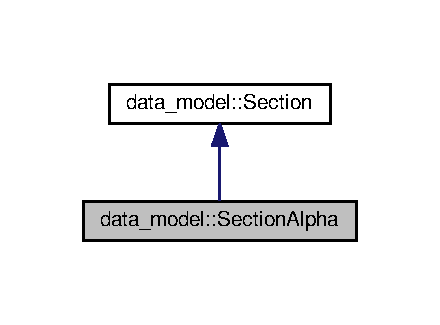
\includegraphics[width=211pt]{classdata__model_1_1_section_alpha__inherit__graph}
\end{center}
\end{figure}


Collaboration diagram for data\+\_\+model\+:\+:Section\+Alpha\+:
\nopagebreak
\begin{figure}[H]
\begin{center}
\leavevmode
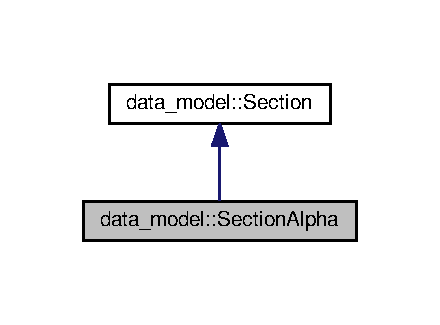
\includegraphics[width=211pt]{classdata__model_1_1_section_alpha__coll__graph}
\end{center}
\end{figure}
\subsection*{Public Member Functions}
\begin{DoxyCompactItemize}
\item 
\hyperlink{classdata__model_1_1_section_alpha_ab2303128daa08e59096fb0914f44f832}{Section\+Alpha} (const std\+::vector$<$ \hyperlink{structdata__model_1_1_result_code}{Result\+Code} $>$ \&, const std\+::vector$<$ \hyperlink{structdata__model_1_1_result_code}{Result\+Code} $>$ \&, const std\+::vector$<$ \hyperlink{structdata__model_1_1_result_code}{Result\+Code} $>$ \&)\hypertarget{classdata__model_1_1_section_alpha_ab2303128daa08e59096fb0914f44f832}{}\label{classdata__model_1_1_section_alpha_ab2303128daa08e59096fb0914f44f832}

\begin{DoxyCompactList}\small\item\em \hyperlink{classdata__model_1_1_section_alpha}{Section\+Alpha}. \end{DoxyCompactList}\item 
\hyperlink{classdata__model_1_1_section_alpha_aefb4dc9b6b518dcd07047f7deab7766c}{$\sim$\+Section\+Alpha} ()=default\hypertarget{classdata__model_1_1_section_alpha_aefb4dc9b6b518dcd07047f7deab7766c}{}\label{classdata__model_1_1_section_alpha_aefb4dc9b6b518dcd07047f7deab7766c}

\begin{DoxyCompactList}\small\item\em $\sim$\+Section\+Alpha \end{DoxyCompactList}\item 
\hyperlink{classdata__model_1_1_section_acba8f1759f6c20b81bed2d4a1178a155}{Section\+Type} \hyperlink{classdata__model_1_1_section_alpha_a41b854bb12eeb3ac31ccf1f6064fbf46}{Get\+Section\+Type} () const override
\begin{DoxyCompactList}\small\item\em Get\+Section\+Type. \end{DoxyCompactList}\item 
void \hyperlink{classdata__model_1_1_section_alpha_ac75f740b6bee40f4f154792c2ee2f79d}{Add\+C\+Dim} (\hyperlink{structdata__model_1_1_result_code}{Result\+Code})\hypertarget{classdata__model_1_1_section_alpha_ac75f740b6bee40f4f154792c2ee2f79d}{}\label{classdata__model_1_1_section_alpha_ac75f740b6bee40f4f154792c2ee2f79d}

\begin{DoxyCompactList}\small\item\em Add\+C\+Dim. \end{DoxyCompactList}\item 
void \hyperlink{classdata__model_1_1_section_alpha_ad39e907fadc2c3ec712d6bb19b78ca99}{Add\+Edge} (\hyperlink{structdata__model_1_1_result_code}{Result\+Code})\hypertarget{classdata__model_1_1_section_alpha_ad39e907fadc2c3ec712d6bb19b78ca99}{}\label{classdata__model_1_1_section_alpha_ad39e907fadc2c3ec712d6bb19b78ca99}

\begin{DoxyCompactList}\small\item\em Add\+Edge. \end{DoxyCompactList}\item 
void \hyperlink{classdata__model_1_1_section_alpha_ae957bfa630fd3afe6c826cfd142966f9}{Add\+Defect} (\hyperlink{structdata__model_1_1_result_code}{Result\+Code})\hypertarget{classdata__model_1_1_section_alpha_ae957bfa630fd3afe6c826cfd142966f9}{}\label{classdata__model_1_1_section_alpha_ae957bfa630fd3afe6c826cfd142966f9}

\begin{DoxyCompactList}\small\item\em Add\+Defect. \end{DoxyCompactList}\item 
size\+\_\+t \hyperlink{classdata__model_1_1_section_alpha_aa2358cc77c3550a0478c3b4d7bce3243}{Get\+C\+Dim\+List\+Size} () const 
\begin{DoxyCompactList}\small\item\em Get\+C\+Dim\+List\+Size. \end{DoxyCompactList}\item 
size\+\_\+t \hyperlink{classdata__model_1_1_section_alpha_aa2549b4e536321e57a16f1091fa1498e}{Get\+Edge\+List\+Size} () const 
\begin{DoxyCompactList}\small\item\em Get\+Edge\+List\+Size. \end{DoxyCompactList}\item 
size\+\_\+t \hyperlink{classdata__model_1_1_section_alpha_a3aa4de03f8a2e085e5c2c27c5a03eac3}{Get\+Defect\+List\+Size} () const 
\begin{DoxyCompactList}\small\item\em Get\+Defect\+List\+Size. \end{DoxyCompactList}\item 
const \hyperlink{structdata__model_1_1_result_code}{Result\+Code} $\ast$ \hyperlink{classdata__model_1_1_section_alpha_aee3028b8f651b2d9a3146d4c9bccdb42}{Get\+C\+Dim\+Element} (unsigned int) const 
\begin{DoxyCompactList}\small\item\em Get\+C\+Dim\+Element. \end{DoxyCompactList}\item 
const \hyperlink{structdata__model_1_1_result_code}{Result\+Code} $\ast$ \hyperlink{classdata__model_1_1_section_alpha_a507f5b4e4a54e32caa7e5f4d166f836d}{Get\+Edge\+Element} (unsigned int) const 
\begin{DoxyCompactList}\small\item\em Get\+Edge\+Element. \end{DoxyCompactList}\item 
const \hyperlink{structdata__model_1_1_result_code}{Result\+Code} $\ast$ \hyperlink{classdata__model_1_1_section_alpha_ae02eec2a868713066f67a6a9b82c9e5b}{Get\+Defect\+Element} (unsigned int) const 
\begin{DoxyCompactList}\small\item\em Get\+Defect\+Element. \end{DoxyCompactList}\end{DoxyCompactItemize}
\subsection*{Additional Inherited Members}


\subsection{Detailed Description}
The \hyperlink{classdata__model_1_1_section_alpha}{Section\+Alpha} class. 

\subsection{Member Function Documentation}
\index{data\+\_\+model\+::\+Section\+Alpha@{data\+\_\+model\+::\+Section\+Alpha}!Get\+C\+Dim\+Element@{Get\+C\+Dim\+Element}}
\index{Get\+C\+Dim\+Element@{Get\+C\+Dim\+Element}!data\+\_\+model\+::\+Section\+Alpha@{data\+\_\+model\+::\+Section\+Alpha}}
\subsubsection[{\texorpdfstring{Get\+C\+Dim\+Element(unsigned int) const }{GetCDimElement(unsigned int) const }}]{\setlength{\rightskip}{0pt plus 5cm}const {\bf Result\+Code} $\ast$ data\+\_\+model\+::\+Section\+Alpha\+::\+Get\+C\+Dim\+Element (
\begin{DoxyParamCaption}
\item[{unsigned int}]{i}
\end{DoxyParamCaption}
) const}\hypertarget{classdata__model_1_1_section_alpha_aee3028b8f651b2d9a3146d4c9bccdb42}{}\label{classdata__model_1_1_section_alpha_aee3028b8f651b2d9a3146d4c9bccdb42}


Get\+C\+Dim\+Element. 

\begin{DoxyReturn}{Returns}

\end{DoxyReturn}
\index{data\+\_\+model\+::\+Section\+Alpha@{data\+\_\+model\+::\+Section\+Alpha}!Get\+C\+Dim\+List\+Size@{Get\+C\+Dim\+List\+Size}}
\index{Get\+C\+Dim\+List\+Size@{Get\+C\+Dim\+List\+Size}!data\+\_\+model\+::\+Section\+Alpha@{data\+\_\+model\+::\+Section\+Alpha}}
\subsubsection[{\texorpdfstring{Get\+C\+Dim\+List\+Size() const }{GetCDimListSize() const }}]{\setlength{\rightskip}{0pt plus 5cm}size\+\_\+t data\+\_\+model\+::\+Section\+Alpha\+::\+Get\+C\+Dim\+List\+Size (
\begin{DoxyParamCaption}
{}
\end{DoxyParamCaption}
) const}\hypertarget{classdata__model_1_1_section_alpha_aa2358cc77c3550a0478c3b4d7bce3243}{}\label{classdata__model_1_1_section_alpha_aa2358cc77c3550a0478c3b4d7bce3243}


Get\+C\+Dim\+List\+Size. 

\begin{DoxyReturn}{Returns}

\end{DoxyReturn}
\index{data\+\_\+model\+::\+Section\+Alpha@{data\+\_\+model\+::\+Section\+Alpha}!Get\+Defect\+Element@{Get\+Defect\+Element}}
\index{Get\+Defect\+Element@{Get\+Defect\+Element}!data\+\_\+model\+::\+Section\+Alpha@{data\+\_\+model\+::\+Section\+Alpha}}
\subsubsection[{\texorpdfstring{Get\+Defect\+Element(unsigned int) const }{GetDefectElement(unsigned int) const }}]{\setlength{\rightskip}{0pt plus 5cm}const {\bf Result\+Code} $\ast$ data\+\_\+model\+::\+Section\+Alpha\+::\+Get\+Defect\+Element (
\begin{DoxyParamCaption}
\item[{unsigned}]{int}
\end{DoxyParamCaption}
) const}\hypertarget{classdata__model_1_1_section_alpha_ae02eec2a868713066f67a6a9b82c9e5b}{}\label{classdata__model_1_1_section_alpha_ae02eec2a868713066f67a6a9b82c9e5b}


Get\+Defect\+Element. 

\begin{DoxyReturn}{Returns}

\end{DoxyReturn}
\index{data\+\_\+model\+::\+Section\+Alpha@{data\+\_\+model\+::\+Section\+Alpha}!Get\+Defect\+List\+Size@{Get\+Defect\+List\+Size}}
\index{Get\+Defect\+List\+Size@{Get\+Defect\+List\+Size}!data\+\_\+model\+::\+Section\+Alpha@{data\+\_\+model\+::\+Section\+Alpha}}
\subsubsection[{\texorpdfstring{Get\+Defect\+List\+Size() const }{GetDefectListSize() const }}]{\setlength{\rightskip}{0pt plus 5cm}size\+\_\+t data\+\_\+model\+::\+Section\+Alpha\+::\+Get\+Defect\+List\+Size (
\begin{DoxyParamCaption}
{}
\end{DoxyParamCaption}
) const}\hypertarget{classdata__model_1_1_section_alpha_a3aa4de03f8a2e085e5c2c27c5a03eac3}{}\label{classdata__model_1_1_section_alpha_a3aa4de03f8a2e085e5c2c27c5a03eac3}


Get\+Defect\+List\+Size. 

\begin{DoxyReturn}{Returns}

\end{DoxyReturn}
\index{data\+\_\+model\+::\+Section\+Alpha@{data\+\_\+model\+::\+Section\+Alpha}!Get\+Edge\+Element@{Get\+Edge\+Element}}
\index{Get\+Edge\+Element@{Get\+Edge\+Element}!data\+\_\+model\+::\+Section\+Alpha@{data\+\_\+model\+::\+Section\+Alpha}}
\subsubsection[{\texorpdfstring{Get\+Edge\+Element(unsigned int) const }{GetEdgeElement(unsigned int) const }}]{\setlength{\rightskip}{0pt plus 5cm}const {\bf Result\+Code} $\ast$ data\+\_\+model\+::\+Section\+Alpha\+::\+Get\+Edge\+Element (
\begin{DoxyParamCaption}
\item[{unsigned int}]{i}
\end{DoxyParamCaption}
) const}\hypertarget{classdata__model_1_1_section_alpha_a507f5b4e4a54e32caa7e5f4d166f836d}{}\label{classdata__model_1_1_section_alpha_a507f5b4e4a54e32caa7e5f4d166f836d}


Get\+Edge\+Element. 

\begin{DoxyReturn}{Returns}

\end{DoxyReturn}
\index{data\+\_\+model\+::\+Section\+Alpha@{data\+\_\+model\+::\+Section\+Alpha}!Get\+Edge\+List\+Size@{Get\+Edge\+List\+Size}}
\index{Get\+Edge\+List\+Size@{Get\+Edge\+List\+Size}!data\+\_\+model\+::\+Section\+Alpha@{data\+\_\+model\+::\+Section\+Alpha}}
\subsubsection[{\texorpdfstring{Get\+Edge\+List\+Size() const }{GetEdgeListSize() const }}]{\setlength{\rightskip}{0pt plus 5cm}size\+\_\+t data\+\_\+model\+::\+Section\+Alpha\+::\+Get\+Edge\+List\+Size (
\begin{DoxyParamCaption}
{}
\end{DoxyParamCaption}
) const}\hypertarget{classdata__model_1_1_section_alpha_aa2549b4e536321e57a16f1091fa1498e}{}\label{classdata__model_1_1_section_alpha_aa2549b4e536321e57a16f1091fa1498e}


Get\+Edge\+List\+Size. 

\begin{DoxyReturn}{Returns}

\end{DoxyReturn}
\index{data\+\_\+model\+::\+Section\+Alpha@{data\+\_\+model\+::\+Section\+Alpha}!Get\+Section\+Type@{Get\+Section\+Type}}
\index{Get\+Section\+Type@{Get\+Section\+Type}!data\+\_\+model\+::\+Section\+Alpha@{data\+\_\+model\+::\+Section\+Alpha}}
\subsubsection[{\texorpdfstring{Get\+Section\+Type() const override}{GetSectionType() const override}}]{\setlength{\rightskip}{0pt plus 5cm}{\bf Section\+Alpha\+::\+Section\+Type} data\+\_\+model\+::\+Section\+Alpha\+::\+Get\+Section\+Type (
\begin{DoxyParamCaption}
{}
\end{DoxyParamCaption}
) const\hspace{0.3cm}{\ttfamily [override]}, {\ttfamily [virtual]}}\hypertarget{classdata__model_1_1_section_alpha_a41b854bb12eeb3ac31ccf1f6064fbf46}{}\label{classdata__model_1_1_section_alpha_a41b854bb12eeb3ac31ccf1f6064fbf46}


Get\+Section\+Type. 

\begin{DoxyReturn}{Returns}

\end{DoxyReturn}


Implements \hyperlink{classdata__model_1_1_section_a06487a79e538e1849bb1838cf6a0875b}{data\+\_\+model\+::\+Section}.



The documentation for this class was generated from the following files\+:\begin{DoxyCompactItemize}
\item 
model/section.\+h\item 
model/section.\+cpp\end{DoxyCompactItemize}

\hypertarget{classdata__model_1_1_section_beta}{}\section{data\+\_\+model\+:\+:Section\+Beta Class Reference}
\label{classdata__model_1_1_section_beta}\index{data\+\_\+model\+::\+Section\+Beta@{data\+\_\+model\+::\+Section\+Beta}}


The \hyperlink{classdata__model_1_1_section_beta}{Section\+Beta} class.  




{\ttfamily \#include $<$section.\+h$>$}



Inheritance diagram for data\+\_\+model\+:\+:Section\+Beta\+:
\nopagebreak
\begin{figure}[H]
\begin{center}
\leavevmode
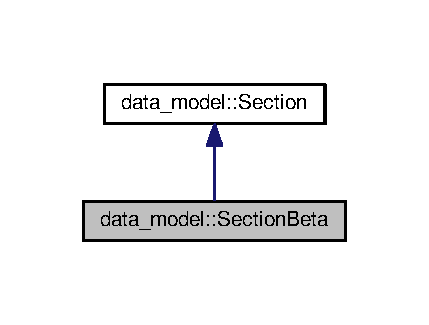
\includegraphics[width=206pt]{classdata__model_1_1_section_beta__inherit__graph}
\end{center}
\end{figure}


Collaboration diagram for data\+\_\+model\+:\+:Section\+Beta\+:
\nopagebreak
\begin{figure}[H]
\begin{center}
\leavevmode
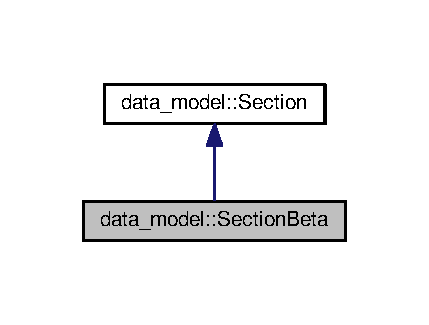
\includegraphics[width=206pt]{classdata__model_1_1_section_beta__coll__graph}
\end{center}
\end{figure}
\subsection*{Public Member Functions}
\begin{DoxyCompactItemize}
\item 
\hyperlink{classdata__model_1_1_section_beta_a8a7b7a25235b6b74e0af3c0857581fb8}{Section\+Beta} (float, float)\hypertarget{classdata__model_1_1_section_beta_a8a7b7a25235b6b74e0af3c0857581fb8}{}\label{classdata__model_1_1_section_beta_a8a7b7a25235b6b74e0af3c0857581fb8}

\begin{DoxyCompactList}\small\item\em \hyperlink{classdata__model_1_1_section_beta}{Section\+Beta}. \end{DoxyCompactList}\item 
\hyperlink{classdata__model_1_1_section_beta_ad06c9ba3d8486a04d8ce3c0d334a2fa4}{$\sim$\+Section\+Beta} ()=default\hypertarget{classdata__model_1_1_section_beta_ad06c9ba3d8486a04d8ce3c0d334a2fa4}{}\label{classdata__model_1_1_section_beta_ad06c9ba3d8486a04d8ce3c0d334a2fa4}

\begin{DoxyCompactList}\small\item\em $\sim$\+Section\+Beta \end{DoxyCompactList}\item 
float \hyperlink{classdata__model_1_1_section_beta_aa21981823334ed9e50eee0fc95dfa4c7}{Get\+Endurance} () const 
\begin{DoxyCompactList}\small\item\em Get\+Endurance. \end{DoxyCompactList}\item 
float \hyperlink{classdata__model_1_1_section_beta_a0ceb4a4bf82c216bea9d021b7e8b8481}{Get\+Elasticity} () const 
\begin{DoxyCompactList}\small\item\em Get\+Elasticity. \end{DoxyCompactList}\item 
\hyperlink{classdata__model_1_1_section_acba8f1759f6c20b81bed2d4a1178a155}{Section\+Type} \hyperlink{classdata__model_1_1_section_beta_a2eb6a17542583ac5d3b1b600cd56a1da}{Get\+Section\+Type} () const override
\begin{DoxyCompactList}\small\item\em Get\+Section\+Type. \end{DoxyCompactList}\end{DoxyCompactItemize}
\subsection*{Additional Inherited Members}


\subsection{Detailed Description}
The \hyperlink{classdata__model_1_1_section_beta}{Section\+Beta} class. 

\subsection{Member Function Documentation}
\index{data\+\_\+model\+::\+Section\+Beta@{data\+\_\+model\+::\+Section\+Beta}!Get\+Elasticity@{Get\+Elasticity}}
\index{Get\+Elasticity@{Get\+Elasticity}!data\+\_\+model\+::\+Section\+Beta@{data\+\_\+model\+::\+Section\+Beta}}
\subsubsection[{\texorpdfstring{Get\+Elasticity() const }{GetElasticity() const }}]{\setlength{\rightskip}{0pt plus 5cm}float data\+\_\+model\+::\+Section\+Beta\+::\+Get\+Elasticity (
\begin{DoxyParamCaption}
{}
\end{DoxyParamCaption}
) const}\hypertarget{classdata__model_1_1_section_beta_a0ceb4a4bf82c216bea9d021b7e8b8481}{}\label{classdata__model_1_1_section_beta_a0ceb4a4bf82c216bea9d021b7e8b8481}


Get\+Elasticity. 

\begin{DoxyReturn}{Returns}

\end{DoxyReturn}
\index{data\+\_\+model\+::\+Section\+Beta@{data\+\_\+model\+::\+Section\+Beta}!Get\+Endurance@{Get\+Endurance}}
\index{Get\+Endurance@{Get\+Endurance}!data\+\_\+model\+::\+Section\+Beta@{data\+\_\+model\+::\+Section\+Beta}}
\subsubsection[{\texorpdfstring{Get\+Endurance() const }{GetEndurance() const }}]{\setlength{\rightskip}{0pt plus 5cm}float data\+\_\+model\+::\+Section\+Beta\+::\+Get\+Endurance (
\begin{DoxyParamCaption}
{}
\end{DoxyParamCaption}
) const}\hypertarget{classdata__model_1_1_section_beta_aa21981823334ed9e50eee0fc95dfa4c7}{}\label{classdata__model_1_1_section_beta_aa21981823334ed9e50eee0fc95dfa4c7}


Get\+Endurance. 

\begin{DoxyReturn}{Returns}

\end{DoxyReturn}
\index{data\+\_\+model\+::\+Section\+Beta@{data\+\_\+model\+::\+Section\+Beta}!Get\+Section\+Type@{Get\+Section\+Type}}
\index{Get\+Section\+Type@{Get\+Section\+Type}!data\+\_\+model\+::\+Section\+Beta@{data\+\_\+model\+::\+Section\+Beta}}
\subsubsection[{\texorpdfstring{Get\+Section\+Type() const override}{GetSectionType() const override}}]{\setlength{\rightskip}{0pt plus 5cm}{\bf Section\+Beta\+::\+Section\+Type} data\+\_\+model\+::\+Section\+Beta\+::\+Get\+Section\+Type (
\begin{DoxyParamCaption}
{}
\end{DoxyParamCaption}
) const\hspace{0.3cm}{\ttfamily [override]}, {\ttfamily [virtual]}}\hypertarget{classdata__model_1_1_section_beta_a2eb6a17542583ac5d3b1b600cd56a1da}{}\label{classdata__model_1_1_section_beta_a2eb6a17542583ac5d3b1b600cd56a1da}


Get\+Section\+Type. 

\begin{DoxyReturn}{Returns}

\end{DoxyReturn}


Implements \hyperlink{classdata__model_1_1_section_a06487a79e538e1849bb1838cf6a0875b}{data\+\_\+model\+::\+Section}.



The documentation for this class was generated from the following files\+:\begin{DoxyCompactItemize}
\item 
model/section.\+h\item 
model/section.\+cpp\end{DoxyCompactItemize}

%--- End generated contents ---

% Index
\backmatter
\newpage
\phantomsection
\clearemptydoublepage
\addcontentsline{toc}{chapter}{Index}
\printindex

\end{document}
